\documentclass[journal,12pt,twocolumn]{IEEEtran}
%
\makeatletter
\makeatother
\usepackage{setspace}
\usepackage{gensymb}
\usepackage{xcolor}
\usepackage{caption}
%\usepackage{stackengine}
%\usepackage{subcaption}
%\doublespacing
\singlespacing



\usepackage{graphicx}
\graphicspath{ {./images}  }
%\usepackage{amssymb}
%\usepackage{relsize}
\usepackage[cmex10]{amsmath}
\usepackage{mathtools}
%\usepackage{amsthm}
%\interdisplaylinepenalty=2500
%\savesymbol{iint}
%\usepackage{txfonts}
%\restoresymbol{TXF}{iint}
\usepackage{wasysym}
\usepackage{amsthm}
\usepackage{mathrsfs}
\usepackage{txfonts}
\usepackage{stfloats}
\usepackage{cite}
\usepackage{cases}
\usepackage{mathtools}
\usepackage{subfig}
\usepackage{enumerate}	
\usepackage{enumitem}
\usepackage{amsmath}
%\usepackage{xtab}
\usepackage{longtable}
\usepackage{multirow}
%\usepackage{algorithm}
%\usepackage{algpseudocode}
\usepackage{enumitem}
\usepackage{mathtools}
%\usepackage{iithtlc}
%\usepackage[framemethod=tikz]{mdframed}
\usepackage{listings}
\usepackage{listings}
    \usepackage[latin1]{inputenc}                                 %%
    \usepackage{color}                                            %%
    \usepackage{array}                                            %%
    \usepackage{longtable}                                        %%
    \usepackage{calc}                                             %%
    \usepackage{multirow}                                         %%
    \usepackage{hhline}                                           %%
    \usepackage{ifthen}                                           %%
  %optionally (for landscape tables embedded in another document): %%
    \usepackage{lscape}     



%\usepackage{stmaryrd}


%\usepackage{wasysym}
%\newcounter{MYtempeqncnt}
\DeclareMathOperator*{\Res}{Res}
%\renewcommand{\baselinestretch}{4}
%\setcounter{secnumdepth}{4}
\renewcommand\thesection{\arabic{section}}
\renewcommand\thesubsection{\thesection.\arabic{subsection}}
\renewcommand\thesubsubsection{\thesubsection.\arabic{subsubsection}}
%\renewcommand\thesubsubsubsection{\thesubsubsection.\arabic{subsubsubsection}}

%\renewcommand\thesectiondis{\arabic{section}}
%\renewcommand\thesubsectiondis{\thesectiondis.\arabic{subsection}}
%\renewcommand\thesubsubsectiondis{\thesubsectiondis.\arabic{subsubsection}}
%\renewcommand\thesubsubsubsectiondis{\thesubsubsectiondis.\arabic{subsubsubsection}}
% correct bad hyphenation here
\hyphenation{op-tical net-works semi-conduc-tor}

%\lstset{
%language=C,
%frame=single, 
%breaklines=true
%}

%\lstset{
	%%basicstyle=\small\ttfamily\bfseries,
	%%numberstyle=\small\ttfamily,
	%language=Octave,
	%backgroundcolor=\color{white},
	%%frame=single,
	%%keywordstyle=\bfseries,
	%%breaklines=true,
	%%showstringspaces=false,
	%%xleftmargin=-10mm,
	%%aboveskip=-1mm,
	%%belowskip=0mm
%}

%\surroundwithmdframed[width=\columnwidth]{lstlisting}
\def\inputGnumericTable{}                                 %%
\lstset{
language=C,
frame=single, 
breaklines=true
}
 

\begin{document}
%

\theoremstyle{definition}
\newtheorem{theorem}{Theorem}[section]
\newtheorem{problem}{Problem}
\newtheorem{proposition}{Proposition}[section]
\newtheorem{lemma}{Lemma}[section]
\newtheorem{corollary}[theorem]{Corollary}
\newtheorem{example}{Example}[section]
\newtheorem{definition}{Definition}[section]
%\newtheorem{algorithm}{Algorithm}[section]
%\newtheorem{cor}{Corollary}
\newcommand{\BEQA}{\begin{eqnarray}}
\newcommand{\EEQA}{\end{eqnarray}}
\newcommand{\define}{\stackrel{\triangle}{=}}

\bibliographystyle{IEEEtran}
%\bibliographystyle{ieeetr}

\providecommand{\nCr}[2]{\,^{#1}C_{#2}} % nCr
\providecommand{\nPr}[2]{\,^{#1}P_{#2}} % nPr
\providecommand{\mbf}{\mathbf}
\providecommand{\pr}[1]{\ensuremath{\Pr\left(#1\right)}}
\providecommand{\qfunc}[1]{\ensuremath{Q\left(#1\right)}}
\providecommand{\sbrak}[1]{\ensuremath{{}\left[#1\right]}}
\providecommand{\lsbrak}[1]{\ensuremath{{}\left[#1\right.}}
\providecommand{\rsbrak}[1]{\ensuremath{{}\left.#1\right]}}
\providecommand{\brak}[1]{\ensuremath{\left(#1\right)}}
\providecommand{\lbrak}[1]{\ensuremath{\left(#1\right.}}
\providecommand{\rbrak}[1]{\ensuremath{\left.#1\right)}}
\providecommand{\cbrak}[1]{\ensuremath{\left\{#1\right\}}}
\providecommand{\lcbrak}[1]{\ensuremath{\left\{#1\right.}}
\providecommand{\rcbrak}[1]{\ensuremath{\left.#1\right\}}}
\theoremstyle{remark}
\newtheorem{rem}{Remark}
\newcommand{\sgn}{\mathop{\mathrm{sgn}}}
\providecommand{\abs}[1]{\left\vert#1\right\vert}
\providecommand{\res}[1]{\Res\displaylimits_{#1}} 
\providecommand{\norm}[1]{\lVert#1\rVert}
\providecommand{\mtx}[1]{\mathbf{#1}}
\providecommand{\mean}[1]{E\left[ #1 \right]}
\providecommand{\fourier}{\overset{\mathcal{F}}{ \rightleftharpoons}}
%\providecommand{\hilbert}{\overset{\mathcal{H}}{ \rightleftharpoons}}
\providecommand{\system}{\overset{\mathcal{H}}{ \longleftrightarrow}}
	%\newcommand{\solution}[2]{\textbf{Solution:}{#1}}
\newcommand{\solution}{\noindent \textbf{Solution: }}
\providecommand{\dec}[2]{\ensuremath{\overset{#1}{\underset{#2}{\gtrless}}}}
\DeclarePairedDelimiter{\ceil}{\lceil}{\rceil}
%\numberwithin{equation}{subsection}
\numberwithin{equation}{section}
%\numberwithin{problem}{subsection}
%\numberwithin{definition}{subsection}
%\makeatletter
%\@addtoreset{figure}{section}
%\makeatother

\let\StandardTheFigure\thefigure
%\renewcommand{\thefigure}{\theproblem.\arabic{figure}}
%\renewcommand{\thefigure}{\thesection}


%\numberwithin{figure}{subsection}

%\numberwithin{equation}{subsection}
%\numberwithin{equation}{section}
%\numberwithin{equation}{problem}
%\numberwithin{problem}{subsection}
%\numberwithin{problem}{section}
%%\numberwithin{definition}{subsection}
%\makeatletter
%\@addtoreset{figure}{problem}
%\makeatother
%\makeatletter
%\@addtoreset{table}{problem}
%\makeatother

\let\StandardTheFigure\thefigure
\let\StandardTheTable\thetable
%%\renewcommand{\thefigure}{\theproblem.\arabic{figure}}
%\renewcommand{\thefigure}{\theproblem}

%%\numberwithin{figure}{section}

%%\numberwithin{figure}{subsection}



\def\putbox#1#2#3{\makebox[0in][l]{\makebox[#1][l]{}\raisebox{\baselineskip}[0in][0in]{\raisebox{#2}[0in][0in]{#3}}}}
     \def\rightbox#1{\makebox[0in][r]{#1}}
     \def\centbox#1{\makebox[0in]{#1}}
     \def\topbox#1{\raisebox{-\baselineskip}[0in][0in]{#1}}
     \def\midbox#1{\raisebox{-0.5\baselineskip}[0in][0in]{#1}}



\title{ 
%	\logo{
Modern Synchronization Techniques for Reliable Communication 
%	}
}



\author{Theresh Babu Benguluri and G V V Sharma$^{*}$% <-this % stops a space
\thanks{*The authors are with the Department
of Electrical Engineering, Indian Institute of Technology, Hyderabad
502285 India e-mail:  gadepall@iith.ac.in.}
}


% make the title area
\maketitle

\tableofcontents

%\bigskip
%
%\begin{abstract}
%%\boldmath
%A brief description about the modulation/demodulation blocks and Coding/Decoding blocks for DVBS2.
%% and the Kaiser window is used for the FIR filter.
%\end{abstract}

%\IEEEpeerreviewmaketitle
%
\section{Time Offset: Gardner TED}
%\subsection{Transmitter}
%\begin{equation}
%m \rightarrow\boxed	{BPSK}\rightarrow\boxed	{\uparrow T_{sym}}\rightarrow C	
%\end{equation}
%
%  Let bit stream was $m$, $xc$ will be mapped sequence and $C$ will be upsampled by $T_{sym}$
% Where $T_{sym}$ is the samples per symbol. 
%\begin{equation}
%X=P \circledast C
%\end{equation} where $P$ is the shape of the pulse. And defined as,
%\begin{equation}
%    P =
%    \begin{cases}
%      1 & 0\leq t\leq 99 \\
%      0        & otherwise
%    \end{cases}
%  \end{equation}
%\subsection{Receiver}
Let the $m$th sample in the $r$th received symbol time slot be
\begin{equation}
Y_k(m)= X_k + V_k(m), \quad k = 1,\dots,N, m = 1 ,\dots,M.
\end{equation} 
where $X_k$ is the transmitted symbol in the $k$th time slot and $V_k(m) \sim \mathcal{N}\brak{0,\sigma^2} $. 
The decision variable for the $k$th symbol 
is
\begin{align}
U_k&=Y_{k-1}\brak{\frac{M}{2}}\sbrak{Y_{k}\brak{M}-Y_{k-1}\brak{M}}
\end{align}
%
\subsection{Plots}
\begin{figure}
\begin{center}
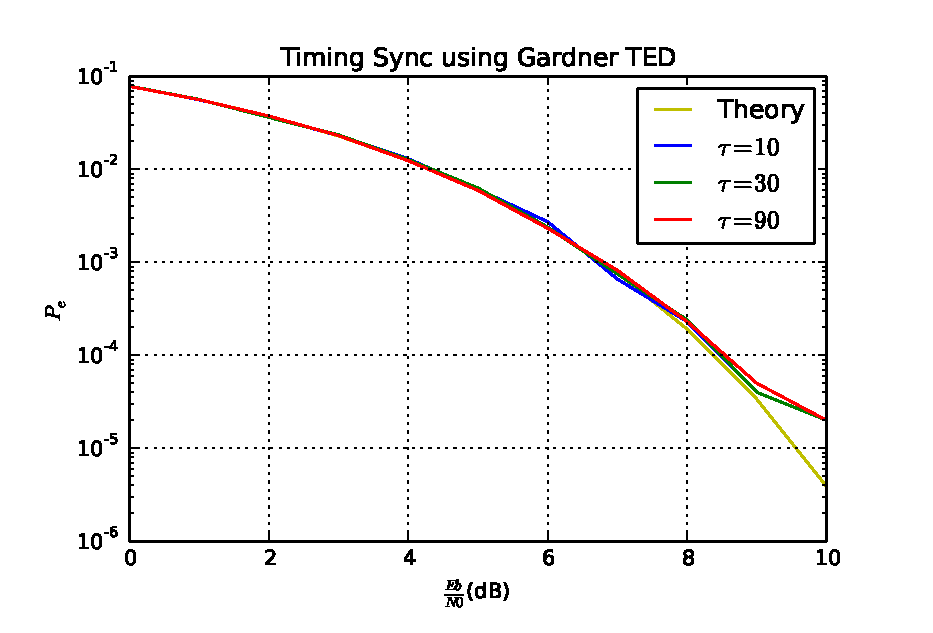
\includegraphics[width=\columnwidth]{./figs/Different_timeoffsets_snrvsber.eps}
\end{center}
\caption{SNR VS BER with different time offsets}
\label{fig:freq_best}
\end{figure}
%
\begin{figure}
\begin{center}
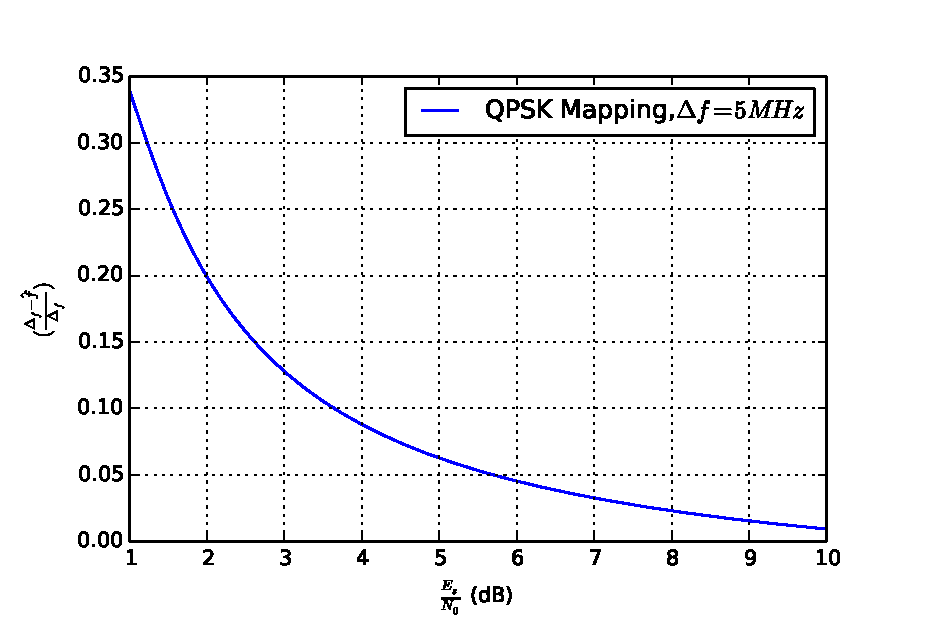
\includegraphics[width=\columnwidth]{./figs/frequencyestiamtion_best_error_vs_snr.eps}
\end{center}
\caption{$\Delta f = 5$ MHz}
\label{fig:freq_est}
\end{figure}

\section{Frequency Offset: LR Technique}
%There are two parts.
%\begin{itemize}
%\item Estimate
%\item Exact
%\end{itemize}
Let the frequency offset be 
$\Delta f$  \cite{1}.  Then
\begin{equation}
\label{eq:freq_offset_model}
Y_k= X_k e^{j2\pi\Delta fkM} + V_k, \quad k = 1,\dots,N 
\end{equation}  
From \eqref{eq:freq_offset_model},
%
\begin{align}
Y_kX_k^*&= \abs{X_k}^2e^{j2\pi\Delta fkM}+ X_k^*{V}_k\\
\implies r_k&=e^{j2\pi\Delta fkM}+ \bar{V}_k
\end{align}
where
\begin{align}
r_k=Y_kX_k^*, \bar{V}_k=X_k^*{V}_k, \abs{X_k}^2=1
\end{align}
%
The autocorrelation can be calculated as
\begin{equation}
R(k) \overset{\Delta}{=} \frac{1}{N-k}\sum_{i=k+1}^{N} r_{i}r^{*}_{i-k}
 , 1 \leq k \leq N-1
\end{equation}
Where N is the length of the received signal.
%DVB-S2 operating with large frequency. So Large frequency offset model has to be employed which is the  Exact approximation of LR technique \cite{1}
For large centre frequency, the following yields a good approximation for frequency offset upto 40 
MHz.
\begin{equation}
\Delta\hat{f} \approx \frac{1}{2\pi M}\frac{\sum_{k=1}^{P}\text{Im}(R(k))}{\sum_{k=1}^{P}k\text{Re}(R(k))},
\quad  P\Delta{f}M << 1
\label{eq:Z}
\end{equation}
%
where $P$ is the number of pilot symbols.
\subsection{Plots}
%
The number of pilot symbols is $P = 18$. The codes for generating the plots are available at

Fig. \ref{fig:freq_best} shows the variation of the error in the offset estimate with respect to the offset 
$\Delta f$ when the SNR = 10 dB.  Similarly Fig. \ref{fig: freq_est} shows the variation of the error with 
respect 
to the SNR for $\Delta f = 5 MHz$.
\begin{figure}
\begin{center}
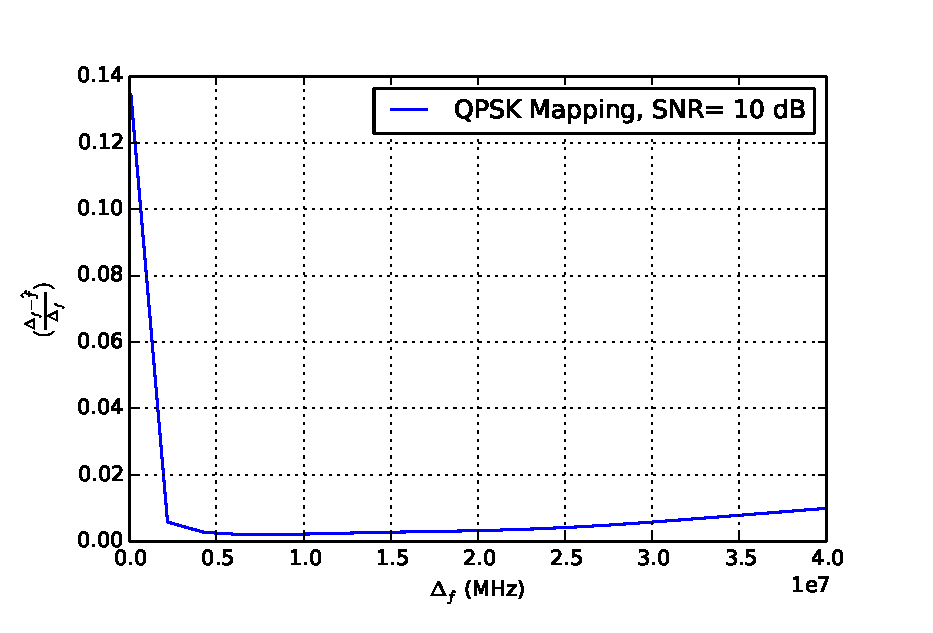
\includegraphics[width=\columnwidth]{./figs/frequency_best.eps}
\end{center}
\caption{Error variation with respect to frequency offset.  }
\label{fig:freq_best}
\end{figure}
%
\begin{figure}
\begin{center}
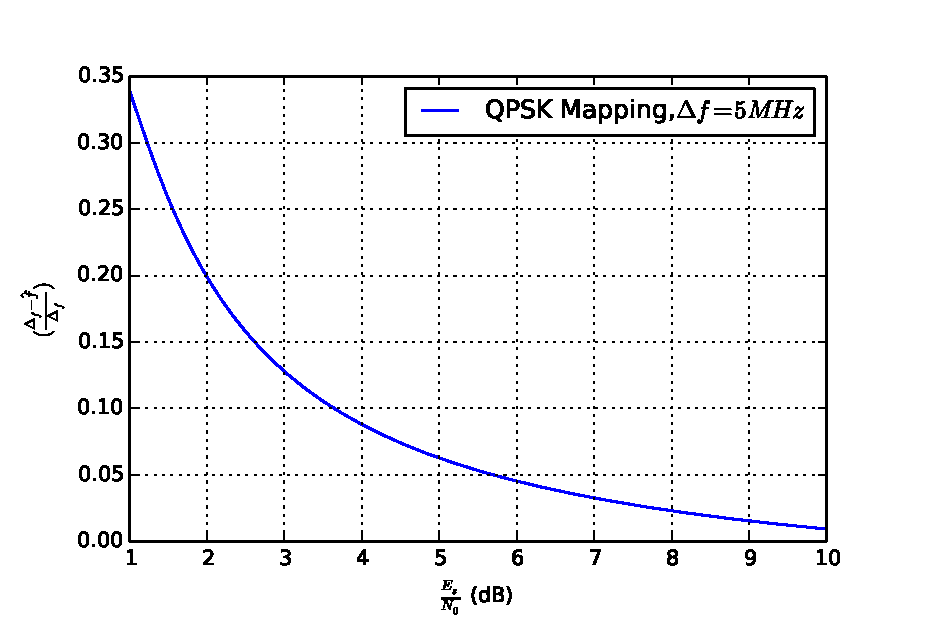
\includegraphics[width=\columnwidth]{./figs/frequencyestiamtion_best_error_vs_snr.eps}
\end{center}
\caption{$\Delta f = 5$ MHz}
\label{fig:freq_est}
\end{figure}


\section{Phase Offset: Feed Forward Maximum Likelihood (FFML)technique}
%There are two parts.
%\begin{itemize}
%\item Estimate
%\item Exact
%\end{itemize}
Let the phase offset be 
$\Delta\phi$  \cite{1}.  Then
\begin{equation}
\label{eq:phase_offset_model}
Y_k= X_k e^{j2\pi\Delta \phi kM} + V_k, \quad k = 1,\dots,N 
\end{equation}  
From \eqref{eq:phase_offset_model},
%
\begin{align}
Y_kX_k^*&= \abs{X_k}^2e^{j2\pi\Delta \phi kM}+ X_k^*{V}_k\\
\implies r_k&=e^{j2\pi\Delta \phi kM}+ \bar{V}_k
\end{align}
where
\begin{align}
r_k=Y_kX_k^*, \bar{V}_k=X_k^*{V}_k, \abs{X_k}^2=1
\end{align}
$\hat{\phi}$ can be written as: 
\begin{equation}
\label{eq:phase_estimation}
\hat{\phi}_k  = arg(r_k)
\end{equation} 

This equation gives the final estimation of phase
\begin{equation}
{\hat{\theta}^{(p)}}_{f}(l) = {\hat{\theta}^{(p)}}_{f}(l-1) + \alpha{SAW}[{\hat{\theta}^{(p)}}_{f}(l) -{\hat{\theta}^{(p)}}_{f}(l-1)] 
\end{equation}
 Where SAW is a saw tooth non-linearity and $\alpha$ $<=1$
 
\subsection{Plots}
\begin{figure}
\begin{center}
\includegraphics[width=\columnwidth]{./figs/Phase_error_with_respect_to_pilots.eps}
\end{center}
\caption{Error variation with respect to frequency offset.  }
\label{fig:freq_best}
\end{figure}
%
\begin{figure}
\begin{center}
\includegraphics[width=\columnwidth]{./figs/Phase_error_with_respect_to_SNR_fixed_pilot.eps}
\end{center}
\caption{$\Delta f = 5$ MHz}
\label{fig:freq_est}
\end{figure}

\begin{thebibliography}{20}
\bibitem{1}
M. Luise and R. Reggiannini:'Carrier frequency recovery in all-digital modems for burst mode transmissions,' IEEE Trans. Commun., vol. 43,
no. 2/3/4, pp. 1169-1178, Feb/Mar/Apr 1995.

\bibitem{2}
U. Mengali and A. N. D'Andrea:'synchronization Techniques for Digital Receivers,' New York: Plenum, 1997.


\end{thebibliography}
\end{document}

